\section{System Modeling and Design}

\subsection{Modeling Steady-State Decode}
\label{sec:modeling_decode}

We present a latency model for LLM decode under three expert management strategies: naive caching, predictive prefetching, and cache-conditional routing.  

We define the following quantities. Qwen3-30B-A3B \cite{yang2025qwen3technicalreport} has $L = 48$ MoE layers, each activating $K = 8$ of 128 experts per layer per token, giving $E = K \cdot L = 384$ expert invocations per token. Each expert is the same size, which for the quantized version, Qwen3-30B-A3B-AWQ~\cite{QuixiAIQwen3AWQ}, is $\sim$2.5 MB. We denote by $T_{ceil}$ the per-token latency when all experts are resident in unified system memory, including both the time spent loading weights from unified memory to the iGPU and compute time. Each expert that must be loaded from SSD incurs a cost $T_{SSD, n}$ , where $n$ is the number of concurrent expert loads. The analytical models in this section assume that background SSD transfers do not interfere with inference compute. 

\subsubsection{Baseline SSD-Backed Decode Model}
\label{sec:baseline_model}

We first model a baseline decode implementation in which expert loads are fully synchronous. For each expert invocation, the expert request either hits in the unified memory expert cache or misses and stalls the decode thread until the expert is fetched from SSD. Let $h \in [0,1]$ be the cache hit rate, so that the number of blocking misses per token is $E_{miss} = E \cdot (1 - h)$. The per-token latency is

\begin{equation}
    T_{0} = T_{ceil} +  E_{miss} \cdot T_{SSD,n}.
    \label{eq:lru}
\end{equation}

This model assumes that each blocking expert load contributes independently to decode latency and that SSD transfers cannot overlap with computation and always block the decode path. Figure~\ref{fig:timeline_blocking} illustrates this process with a toy 2-layer MoE LLM.

\begin{figure}[h]
    \centering
    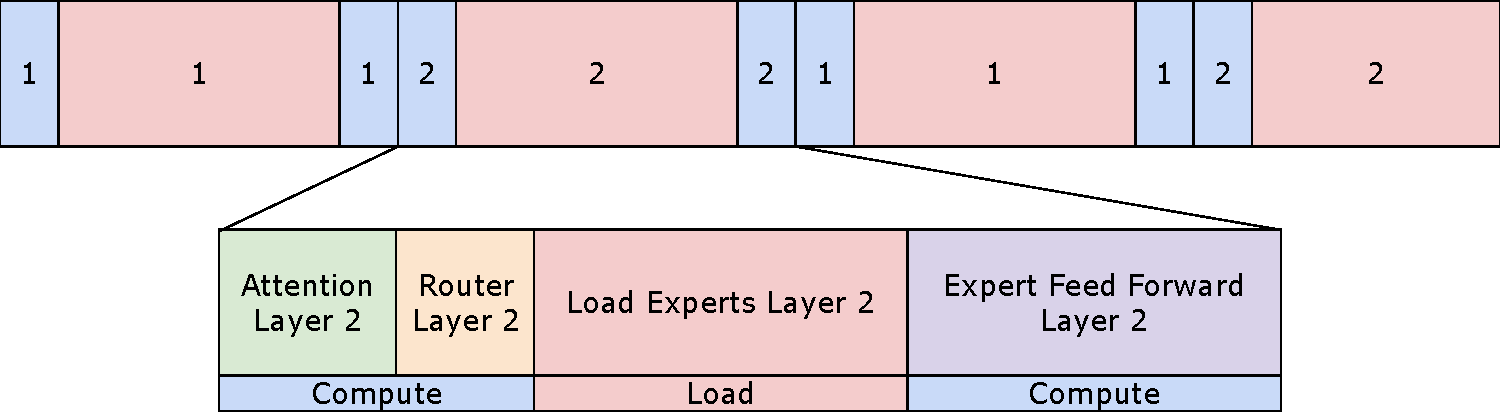
\includegraphics[width=\columnwidth]{figures/timeline_LRU_cropped.pdf}
    \vspace{-10pt}
    \caption{Timeline of decode with blocking expert loads. No predictive prefetch leads to reactive SSD loads on misses}
    \label{fig:timeline_blocking}
\end{figure}


\subsubsection{Predictive Prefetching} 
\label{sec:prefetch}

Predictive prefetching aims to reduce blocking loads by loading predicted experts into a per-layer expert cache of size $C$ proactively: the predictor has a stride, $S$, such that it fires once every $S$ tokens, and issues asynchronous SSD loads for experts likely to be used to generate the next $S$ tokens. If the loads finish before those experts are needed, they are already resident in the cache and no blocking stalls occur, as illustrated in Figure~\ref{fig:timeline_prefetch}. 

On each predictor invocation, up to $B$ prefetch loads (prefetch budget) are issued per layer, for a total issue budget of $M_{issue} = L \cdot B$ loads every $S$ tokens. Not all issued loads are useful: let $\pi \in [0,1]$ be the \emph{precision}, the fraction of prefetched experts that actually get requested by the router. Conversely, let $\rho \in [0,1]$ be the \emph{recall}, the fraction of experts that will be requested by the router on subsequent decode steps that the predictor correctly identified. Low precision wastes SSD bandwidth on unneeded loads; low recall increases cache misses, causing blocking loads from SSD. 

After the predictor runs, the ideal theoretical window to hide asynchronous SSD loads is  $S \cdot T_{ceil}$ ms, the compute time of the next $S$ tokens. This assumes an ideal predictive prefetching schedule where the earliest activated experts are loaded first. It should be noted that if all layers are issuing loads, we will saturate SSD bandwidth and cannot use the entire $S \cdot T_{ceil}$ ms window. We assume no bandwidth contention and that each expert takes $T_{SSD,n}$ ms to load, giving a maximum load hiding capacity:

\begin{equation}
    M_{cap} = \frac{S \cdot T_{ceil} }{T_{SSD, n}}.
    \label{eq:mcap}
\end{equation}

Let $U(S)$ be the number of expert misses that will occur over the next $S$ tokens. There are four constraining dimensions which limit how many experts can be successfully prefetched (hidden and correct) during the decode process of the next $S$ tokens:
\begin{enumerate}
\label{list:constraints}
    \item $\rho \cdot U(S) $: Number of future router requests that are predicted, not including those already in the cache
    \item $\pi \, L B $: Number of useful predictions that are issued, not including predicted experts already in the cache 
    \item $M_{cap}$: The number of prefetches that can complete within the available overlap window
    \item $C$: Number of experts that can be stored in the unified memory expert cache
\end{enumerate}

% This allows us to construct 

% \begin{equation}
%     M_{prefetch} = \min\!\left(\rho \, U(S) \cdot (1-h),\; \pi \, L B \cdot (1-h),\; M_{cap}, \, C\right).
%     \label{eq:mprefetch}
% \end{equation}


\begin{figure}[h]
    \centering
    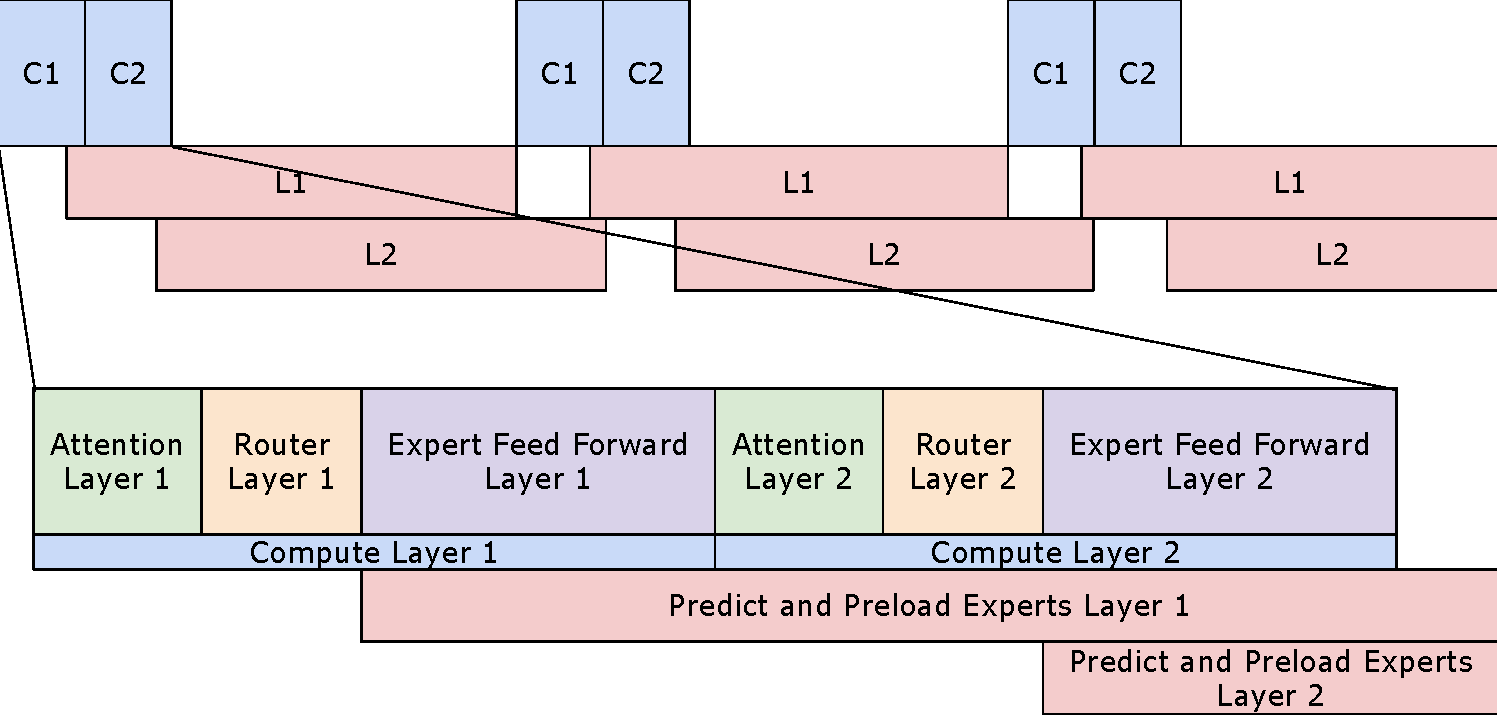
\includegraphics[width=\columnwidth]{figures/timeline_prefetch_cropped.pdf}
    \vspace{-10pt}
    \caption{Timeline of ExpertAhead decode. Predictive prefetches are launched asynchronously and overlap with computation and other prefetches to saturate SSD bandwidth}
    \label{fig:timeline_prefetch}
\end{figure}


\subsubsection{Cache-Conditional Routing}
\label{sec:cc}

Prefetching attempts to load all the experts required for the next token into the expert cache before they are requested by the router. However, imperfect predictor recall means that some experts inevitably cannot be prefetched.  Cache-conditional routing \cite{skliar2025mixturecacheconditionalexpertsefficient} addresses this: rather than executing a decode blocking SSD load for an expert not in memory, this policy allows experts already resident in the cache to replace low priority router-selected experts, avoiding paying a latency penalty of $T_{SSD,n}$.  More generally, cache-conditional routing raises the effective hit rate from $h$ to $h_{eff}$. Therefore, cache misses and thus total SSD traffic are reduced as seen in Equation~\ref{eq:route_miss}.

\begin{equation}
    E_{miss}^{'} = E \cdot \left(1 - h_{eff}\right).
    \label{eq:route_miss}
\end{equation}

\subsubsection{Unified Model}
Predictive prefetching attempts to predict future expert requests and load experts into system memory before they are needed. Cache-conditional routing further reduces blocking loads by allowing low-priority router-selected experts to be substituted with experts already resident in cache.

Together, these mechanisms reduce both the total number of SSD-resident expert loads and the fraction of those loads that appear on the critical decode path, represented as $E_{block} = E_{miss}^{'} - E_{prefetch}$.

\begin{equation}
    \label{eq:unified_full}
    T =
    T_{ceil}
    +
    E_{block} \cdot T_{SSD,n} \,\,\,\,
\end{equation}

This formulation captures the central systems tradeoff explored in this work. Cache-conditional routing reduces total SSD traffic by decreasing the number of required expert fetches, while predictive prefetching overlaps SSD traffic with computation. Together, these mechanisms attack two distinct dimensions of the SSD bottleneck: traffic volume and blocking load latency.

These latency models provide a framework for understanding how predictor accuracy, prediction stride, prefetch budget, and cache capacity influence decode throughput, motivating our system design and experiments in the following sections.

\subsection{Runtime Architecture}
We implement a full-stack MoE inference runtime for an AWQ \cite{lin2026awqactivationawareweightquantization} quantized model: Qwen3-30B-A3B-AWQ \cite{QuixiAIQwen3AWQ}, consisting of a Python control layer connected to a C++/LibTorch~\cite{pytorch} execution backend using pybind \cite{pybind11}. The backend executes the complete autoregressive pipeline using custom ROCm/HIP \cite{rocm} kernels. All experts use W4A16 quantization, with 4-bit weights and BF16 activations. Decode uses a fused GEMV kernel while prefill uses tiled GEMM kernels with on-the-fly dequantization. Expert weights are stored on SSD in a custom packed binary format which allows all weights for a single expert to be read with one \texttt{preadv} call. At runtime, each MoE layer maintains a cache of up to $C$ experts in unified system memory. A predicted or required expert not currently resident in one of these $C$ slots must be fetched from SSD before the forward pass can proceed.  

\subsection{ExpertAhead Predictive Prefetching} 

\subsubsection{Predictor Model}
\label{sec:predictor}
We introduce the ExpertAhead predictor, a lightweight predictor that operates during generation to compute relevance scores for all experts across the next $S$ decode steps. The complete 48-layer predictor ensemble occupies $\sim$72 MB, adding only $\sim$0.4\% overhead to the 16.8 GB model.

The predictor has three distinct input features: \\
1) \textbf{Markov Branch:} Inspired by the EAM approach used in \cite{xue2025moeinfinityefficientmoeinference}, a static first-order Markov matrix $\mathbf{M} \in \mathbb{R}^{128 \times 128}$, computed from training traces, multiplies the current multi-hot expert vector, followed by a linear projection. \\
2) \textbf{Embedding Branch:} Inspired by inter-layer predictors \cite{song2025promoefastmoebasedllm, zhang2026duoservemoedualphaseexpertprefetch, yi2025edgemoeempoweringsparselarge, gavhane2025moebeyondlearningbasedexpertactivation,eliseev2023fastinferencemixtureofexpertslanguage, zhu2026daliworkloadawareoffloadingframework, fang2025fatefastedgeinference, yao2024exploitinginterlayerexpertaffinity} we process the previous $H$ token embeddings via a small 2-layer, 4-head Transformer. The predictor outputs a relevance score for each expert over the next $S$ tokens, and prefetches the $B$ experts with the largest scores (top-$B$). \\
3) \textbf{Prefill Branch:} We hypothesize that generations exhibit similar expert utilization patterns to their prompts, so we feed prefill expert activation distribution into an MLP.  \\

\begin{figure}[h]
    \centering
    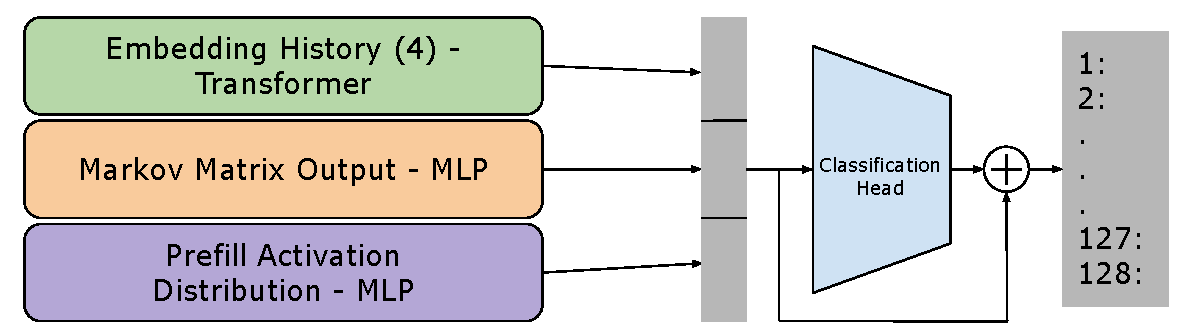
\includegraphics[width=\columnwidth]{figures/predictor_arch (1)_cropped.pdf}
    \vspace{-10pt}
    \caption{ExpertAhead Predictor Architecture}
    \label{fig:expertAhead_pred_arch}
    \vspace{-5pt}
\end{figure}

\subsubsection{Model Training Procedure}

Training data is collected by feeding chunks from the WikiText-103 training set \cite{merity2016pointersentinelmixturemodels} as prompts to Qwen3-30B-A3B-AWQ and recording the hidden-state embeddings and expert-activation traces during prefill and greedy decode. One predictor is trained independently per layer and per stride $S$.

\subsubsection{Runtime Integration}
\label{sec:prefetch_runtime}
Every $S$ decode steps, the predictor asynchronously ranks experts for the next $S$ tokens. Memory-resident experts among the top-$B$ predictions have their timestamps refreshed to prevent eviction. Non-resident experts are assigned victim slots via a least-frequently-recently-used (LFRU) policy and fetched via parallel, asynchronous SSD loads. Cache misses during actual routing trigger blocking loads, and any incomplete prefetch requests are discarded before the next predictor invocation to prevent stale workload backlog.

\subsection{Cache-Conditional Expert Selection}
To reduce the total number of SSD loads, \citet{skliar2025mixturecacheconditionalexpertsefficient} proposes an implementation of cache-conditional expert selection, evaluated on a mobile SoC. The modified router logits are defined as:

\begin{equation}
    \label{eq:top_j}
    z' = z + \lambda \cdot \Delta_{avg} \cdot \tilde{m}_t
\end{equation}


where $z$ are the original router logits, $\lambda$ is a tunable cache-bias strength parameter, and $\tilde{m}_t$ is a binary cache-residency mask indicating whether each expert is currently resident in system memory. The scaling factor $\Delta_{avg}$ normalizes the cache bias relative to the natural spread of the router logits, computed as an exponentially weighted moving average across forward passes.

In this work, we use $\lambda \in \{0,1\}$ and compare different values for top-J expert selection: the $J$ highest-scoring experts selected by the router are always activated, while the remaining $K-J$ expert slots become eligible for substitution with cache-resident experts to reduce SSD traffic. 


\subsection{Target Hardware}

We evaluate our methods on an AMD Ryzen AI 9 HX 370 (Strix Point) SoC. It includes a 12-core Zen 5 CPU and an AMD Radeon 890M integrated GPU sharing 28 GB of unified memory ($\sim$120 GB/s peak) and a peak achievable SSD bandwidth of $\sim$1.5 GB/s measured with an expert loading benchmark.